\documentclass[12pt]{article}
\usepackage[utf8]{inputenc}
\usepackage[margin=1in,bottom=1.5in,a4paper]{geometry}
\usepackage{tikz}
\usepackage{amsmath}
\usepackage{amssymb}
\usepackage{multicol}
\usepackage{xcolor}
\usepackage{tabularx}
\usepackage{mathtools}
\usepackage{ textcomp }
\usepackage{graphicx}
\usepackage{ stmaryrd }
\usepackage{hyperref}
\usepackage{ marvosym }
\usepackage{ dsfont }
\usepackage{ulem}
\tolerance=1000
\usepackage{fancyhdr}
\pagestyle{fancy}
\headheight 50pt

\renewcommand{\thesection}{\Alph{section}}

%edit header and footer
\fancypagestyle{firstpage}{
  \lhead{X-as-a-Service cloud assets}
  \chead{\textbf{\Large Azure}}
  \rhead{CySec Project '21}
}
\lhead{}
\rhead{X-as-a-Service cloud assets}

\cfoot{}
\rfoot{\small\thepage}

\begin{document}
\thispagestyle{firstpage}

\section*{Azure for Students}
Overview on Azure and their services (kinda ranked after use-cases)
\begin{enumerate}
    \item Compute: VMs (IaaS), Container Instances (virtualised Applicationenvironments), App Service, Functions
    \item Networking (VPN,...)
    \item Storage
    \item Mobile services (apps,...)
    \item Databases
    \item Web (Web apps, ...)
    \item IoT (manage all IoT assets, ...)
    \item BigData (cluster services, ...)
    \item AI services and Machine Learning
    \item DevOps
\end{enumerate}


\subsection*{Notes}
\begin{itemize}
    \item CA from my static website: Microsoft Azure TLS Issuing CA 01
    \item Easy to differentiate between VM and Containers: VM virtualise the hardware, containers the OS
    \item \verb|azurewebsites.net|, \verb|azurestaticapps.net| as domain ending
    \item Static and web apps can be set up with the help of Git \\ 
    $\rightarrow$ learning something via Git Accounts?
    \item Possibilities to secure Azure: SecurityCenter, Sentinel, AzureDefender
\end{itemize}

\subsection*{To be checked out:}
\url{https://sonraisecurity.com/blog/attackers-find-aws-s3-bucket-with-17m-users/} \\ \\




\newpage
\subsection*{Most common mistakes with Azure}
\begin{itemize}

    \item \textbf{Misconfiguration of Roles \& Administration:} \footnote{\url{https://blog.e-zest.com/here-are-10-most-common-mistakes-while-managing-azure-cloud}} \footnote{\url{https://www.lightstream.tech/top-5-azure-mistakes-your-security-team-is-making/}} \footnote{\url{https://www.viacode.com/most-common-azure-security-problems/}}
    
    making everyone as (co-)administrator in the Azure subscription. Team members often times remove or delete the Azure components, which creates lot of impact on overall application and ruins the stability of the environment. Members also unknowingly keep on provisioning Azure resources for research and evaluation purpose which causes a huge expenditure. Data Storage Access Misconfig: a user can set permissions that expose data to the entire internet in "Azure Storage" \textbf{(try to do that!)} 

    $\rightarrow$ provide users only with the amount of permission they need to do their job! \\
    RBAC (Role Based Access Control) or ARM (Azure Resource Manager) or MFA (Multi-Factor auth.) 


    \item \textbf{Choosing incorrect specifications (of Azure VM) \& not securing access points} \footnotemark[1] \footnote{\url{https://techgyo.com/5-common-microsoft-azure-security-mistake}} \\
    All aspects like overall user load, nature of the application and geography of the users must be considered by enterprises and individuals hosting their applications, before designing the infrastructure.
    Not securing access points to the clouds, allowing users to access the VM from any machine, anywhere.
    
    
    \item \textbf{Billing of over usage} \footnotemark[1] \\
    They keep running their Azure instances, even if they are not in use or when purpose is served. \\
    $\rightarrow$ keep resources in off-state or delete them once you no longer need them.
    
    
    \item \textbf{Weak, mismanaged Passwords:} \footnotemark[2] \footnotemark[4] \\ 
    Improper password management and bad password habits. Microsoft reports 10 million username/password pair attacks per day.
    
    
    \item \textbf{Misconfig/not enabling of Security/Managing Controls:} \footnotemark[2] \\ 
    Failed to turn on the logging feature. Necessary to permit access visibility but also to see who is accessing and managing the subscription.
    Failing to enable Azures security center and its native security tools (\textbf{check this out!}) \\
    \textbf{TODO}: subnets should not be assigned to a public IP that could open unwanted ports. (Network Security Groups (NSGs)) NSGs control access by permitting or denying network traffic via communication between different workloads on a vNET, network connectivity from on-site environment into Azure, or direct internet connection.
    
    \item \textbf{Lack of Oversight / Security Monitoring:} \footnotemark[2] \footnotemark[3] \\ 
    Missing ongoing management and security (often times just in the beginning and then not covered anymore)
    Security vulnerabilities result when Azure users don’t understand what they are responsible for and the tools and services Azure provides to help them. 
    \begin{center}
        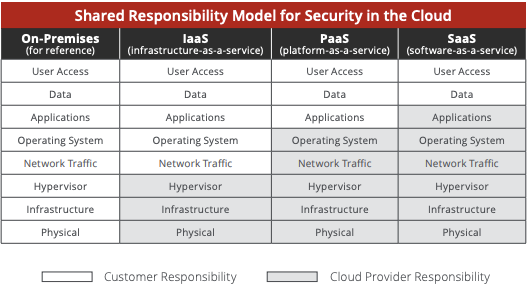
\includegraphics[scale=0.5]{../images/McAfee_Responsibility_Model.png} \footnotemark[5] 
    \end{center}
    
    
    \item \textbf{Cloud misconfiguration:} \footnotemark[3] \\
    Especially the misconfiguration of databases and object storage services. (linked there - \url{https://www.mcafee.com/enterprise/en-us/assets/skyhigh/white-papers/cloud-adoption-risk-report-2019.pdf})
    
    \item \textbf{Not encrypting data at rest:} \footnotemark[3] \\ 
    blobs are encrypted by default, but VM disks are not, creating vuln. User have to enable disk encryption on their own (for free!).
    
    \item \textbf{Not managing patches correctly:} \footnotemark[4] \\
    Not applying a patch at all or do it only half the way.
    
    \item \textbf{Not testing security or taking it for granted:} \footnotemark[4] \footnotemark[1] \\ 
    Users should use penetration testers (microsoft has a policy governing such tests).
    Even though Microsoft secures the platform, it can't protect against e.g. weak passwords
    
    \item \textbf{Not opting for Microsoft support option} \footnotemark[1] \\
    To save costs, companies try to avoid the support when purchasing the Azure subscription. 
    But it can happen, that even a high skilled employer isn't able to e.g. shut down a VM. The support however can do this. If enterprises have not chosen the appropriate support option then there might be a huge impact. 
    
    \item \textbf{McAfee Report} \footnote{\url{https://www.mcafee.com/enterprise/en-us/assets/skyhigh/white-papers/cloud-adoption-risk-report-2019.pdf}} \\
    More and more files contain sensitive information and too many are publicly accessible. Enterprise organizations have an average of 14 misconfigured IaaS/PaaS instances.
    
\end{itemize}


\newpage
\section*{Azure Key Vault}
%\verb|"<your-unique-storage-account-name>" = storageforkeyvault|

%\verb|"<your-unique-keyvault-name>" = super-secure-keyvault|

Search for \verb|.vault.azure.net| websites (e.g. Dorking: \verb|site:*.vault.azure.net/|)\\
$\rightarrow$ no results, aren't listed...

Resolve the key vault uri (\url{https://super-secure-keyvault.vault.azure.net/}, \url{https://aiskeyrun.vault.azure.net}) \\
$\rightarrow$ runs on \verb|51.116.154.67| and \verb|ASN 8075|


%\newpage
\section*{Azure SecurityCenter}
All security recommendations:\\  \url{https://docs.microsoft.com/en-us/azure/security-center/recommendations-reference} \\ \\
\textbf{(Most) Common security recommendations:}
\begin{itemize}
    \item Enable MFA
    \item Secure (management) ports \\ 
    (JIT network access control should be applied on VMs, VMs associated with a NSG, Management ports should be closed on your VMs)
    \item Apply system updates \\
    (60 \% of security breaches caused by vuln's which are already patched)
    \item Remediate Vulnerabilities \\
    (Vulnerabilities in ... should be remediated / Vulnerability assessment should enabled on ...)
    \item Enable encryption at rest
    \item Encrypt data in transit \\
    (... should only be accessible over HTTPS / Only secure connections to ... should be enabled)
    \item Access management and permissions \\
    (RBAC, permissions should be removed from your subscription)
    \item Manage network access \\
    (CORS should not allow every resource to access your ..., Access should be restricted, Remote debugging should be turned off, IP forwarding should be disabled)
    \item Apply DDoS protection
    \item Enable endpoint protection, monitoring agent \& logging \\
    (Monitoring agent should be installed, Diagnostic logs in ... should be enabled)
\end{itemize}


\section*{Azure Storage}
\begin{itemize}
    \item "Data Storage Access Misconfig: a user can set permissions that expose data to the entire internet in Azure Storage" \\ $\rightarrow$ Try to leak something. Can you see that from the outside?
\end{itemize}
Azure Blobs consists of an account and container name with the scheme: \\ \verb|https://{accountName}.blob.core.windows.net/{containerName}|\\ \\
To find open accessible blobs: Google dorking with \verb|site:"*.blob.core.windows.net"| \\
For secondary endpoints: \verb|site:"*-secondary.blob.core.windows.net"| \\ \\
Possible access rights for blobs: \verb|private, blob, container|
\begin{itemize}
    \item Container: \url{https://unprotectedblob.blob.core.windows.net/leakedfiles/Beach.png} is openly accessible
    \item Blob: \url{https://unprotectedblob.blob.core.windows.net/stillleakingfiles/harold.jpeg} is also openly accessible
    \item Private: \url{https://unprotectedblob.blob.core.windows.net/protectedfiles/street.jpg} is protected
\end{itemize}


\section*{Azure Functions}
\url{https://docs.microsoft.com/en-us/azure/azure-functions/functions-overview}
\begin{itemize}
    \item Create functions app with wrong permission and see what you can see.
\end{itemize}

\subsection*{Finding publicly available Azure Functions}
The "vulnerability" for HttpTriggered Functions is to have the \verb|"authLevel"| set to \verb|"anonymous"| in the \verb|function.json|. \\
If this is the case, everyone can execute the function. \\
Examples (for some reason, sometimes the site needs to be reloaded multiple times):
\begin{itemize}
    \item \url{https://tryingtogetaccessfromeverywhere.azurewebsites.net/api/HttpTrigger1}
    \item \url{https://tryingtogetaccessfromeverywhere.azurewebsites.net/api/HttpTrigger1?name=philipp}
\end{itemize}
\begin{center}
    Scheme: \verb|https://{accountName}.azurewebsites.net/api/{functionName}|
\end{center}
However, given an \verb|azurewebsites.net| (e.g. find them via Google dorking: \\ \verb|site:"*.azurewebsites.net"|), we can look for \verb|/api/ + <existing functionnames>| (default one for HttpTriggered: \verb|HttpTrigger1|). \\ \\
For this project we have to know which \verb|azurewebsites.net| belong to which company. Otherwise, we just check for unprotected AzureFunctions. \\ 
Each Azure Function has an own Blob storage with at least two containers called \verb|azure-webjobs-hosts, azure-webjobs-secrets|. \\
The blob storage is then called \verb|"storageaccount<first 5 letters from resourcegroup>| \\ \verb|<4 numbers/digits>"| \\
If someone totally screwed up the settings (i think you can only achieve this with intention) you can find the azure function container via \\ \verb|https://{storageaccount ...}.blob.core.windows.net/{containerName}/| \\ \verb|{resourceGroupName}/<file>|. 
However, we could use dirbuster or crawl to see containers.


%\newpage
\section*{Further ideas}
\begin{itemize}
    \item \url{https://github.com/cyberark/BlobHunter} \\
    Looks like they loop over all existing blob storages in the given account to check if the access level is public. \\
    They get access from the user of the program so they don't analyze from the outside.
    \item \url{https://ninocrudele.com/the-three-most-effective-and-dangerous-cyberattacks-to-azure-and-countermeasures-part-2-attack-the-azure-storage-service}
        \item \url{https://github.com/0xsha/CloudBrute} \\
    Insights so far:
    \begin{itemize}
        \item Checks the domain for used Cloud providers in the HTML
        \item If one is used they check for existing urls, starting with the given keyword concatenated with a dictionary (\verb|storage_small.txt / storage_large.txt|). \\
        E.g. when Azure is used, they search for \\ \verb|<keyword><dictionarywords>.<azureservice>.core.windows.net|
    \end{itemize}
    Seems like we could even extend this by looking for e.g. \verb|.azurewebsites.net|, \verb|.vault.azure.net|
\end{itemize}


\section*{Azure DNSZone}
Nothing to be seen or learned here. \\
Just creating basic DNS entries or setting an IP \textit{(querying the DNS entries is an old finding)}


\section*{azurewebsites.net}
Organization Identifiable Information (OII) and Personally Identifiable Information(PII) is what we are searching for on Azure websites
\begin{itemize}
    \item Can you link \verb|aistestresources.azurewebsites.net| back to AIS? Via DNS/cert./the webpage? 
    
    Certificate: On the first look, you don't see anything. Analyzing the cert of \verb|aistestresources.azurewebsites.net| via different tools and solution, you can't trace back the website to \verb|ais-security.de|

    DNS and the rest is also a dead end
    
    \item Can you link an \verb|azurewebsites.net| url back to a subscription ID or related blob storage or anything else? 
    \begin{itemize}
        \item By checking DNS you get the location of the server which was selected in Azure \\
        E.g. \url{tryingtogetaccessfromeverywhere.azurewebsites.net} is in Germany West-Central
    \end{itemize}

\end{itemize}


\section*{Azure URLs}
\begin{itemize}
	\item \verb|login.windows.net|
	\item \verb|management.azure.com| (Azure API)
	\item \verb|management.core.windows.net| (Azure API)
	\item \verb|azureconnector.deepsecurity.trendmicro.com| (Azure connector 'Quick' option)
\end{itemize}


\section*{Conclusion}
So far, we can identify public available \textit{Azure Functions} and \textit{Blob Storages}. However, we cannot trace them back to a company, a subscription ID, or any other OII or PII.\\
If you have given a company name, you could try to find something via Google Dorking (e.g. \verb|allintext:ais security [more possible keywords here] site:"*.azurewebsites.net"|), however this can't really be automized.

\end{document}
